\documentclass[t]{beamer}
\usepackage[utf8x]{inputenc}
\usepackage{graphicx}

\setbeamercovered{transparent}
\setbeamersize{text margin left=1em, text margin right=0em}
\setbeamertemplate{sidebar right}{}
\setbeamertemplate{footline}{\hfill\insertframenumber{}~~~}
\setbeamercovered{invisible}

\setbeamertemplate{subsection in toc}[square]
\AtBeginSubsection[]
{
 \begin{frame}<beamer>
 \frametitle{Overview}
 \tableofcontents[currentsubsection]
 \end{frame}
}

\usepackage{listings}

\usepackage{listings}
\lstdefinelanguage{ReactiveML}
  {morekeywords={assert,asr,class,closed,constraint,external,%
      functor,include,inherit,land,lazy,lor,lsl,lsr,lxor,method,mod,%
      module,new,open,parser,private,sig,struct,val,virtual,when,%
      object,%
      and,as,begin,do,done,dopar,downto,else,end,exception,for,%
      fun,function,if,in,let,match,mutable,of,rec,then,%
      to,try,type,while,with,%
      process,emit,await,signal,default,gather,present,control,until,%
      loop,nothing,pause,pre,run,immediate,one.last},%
   sensitive,%
   morecomment=[n]{(*}{*)},%
   morestring=[b]",%
   moredelim=*[directive]\#,%
   moredirectives={open,close,include}%
  }[keywords,comments,strings,directives]%

% \lstset{language=ReactiveML,%
%    basicstyle=\ttfamily,%
%    keywordstyle=\bfseries\rmfamily,%
%    columns=fullflexible,%
%    moredelim=[is][\itshape]{\#}{\#}%
% }

\lstset{language=ReactiveML,%
   basicstyle=\ttfamily,%
   keywordstyle=\ttfamily,%
   columns=fullflexible,%
   moredelim=[is][\itshape]{\#}{\#}%
}

% \usepackage{alltt}
% \newenvironment{lstlisting}%
% {\begin{alltt}}%
% {\end{alltt}}

%%% Local Variables: 
%%% mode: latex
%%% TeX-master: "these"
%%% End: 

\lstset{language=ReactiveML,%
   basicstyle=\ttfamily,%
   keywordstyle=\color{blue}\ttfamily,%
   columns=fullflexible,%
   moredelim=[is][\itshape]{\#}{\#},%
   showstringspaces=false,%
}
\lstnewenvironment{lstrml}%
{\footnotesize \lstset{language=ReactiveML,keepspaces=true}}
{}

\title{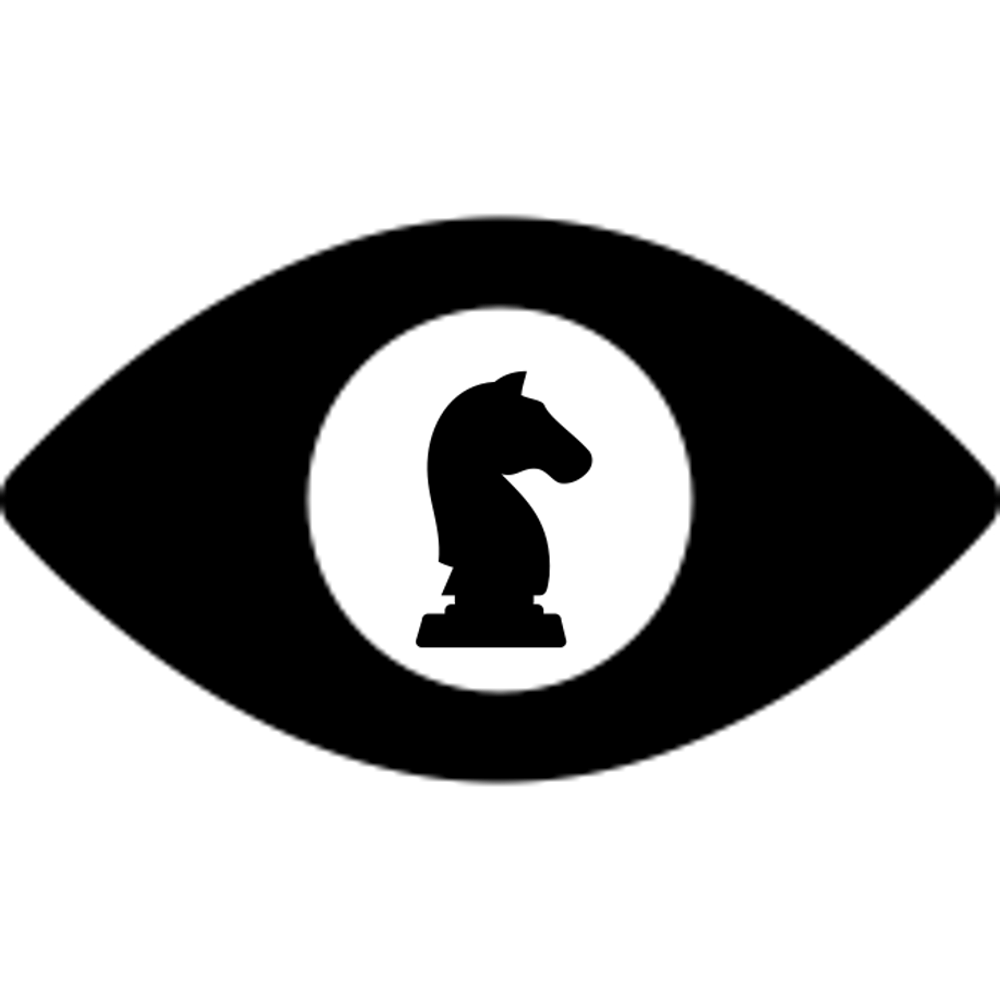
\includegraphics[scale=0.1]{figures/chesseye}
  \\
  ChessEye}
\author{Louis Mandel \and J{\'e}r{\^o}me Sim{\'e}on \and Philippe Suter}
\date{Palaver \\ July 12, 2016}

\begin{document}

%%%%%%%%%%%%%%%%%%%%%%%%%%%%%%%%%%%%%%%%%%%%%%%%%%%%%%%%%%%%%%%%%%%%%%%%%%%

\begin{frame}
  \titlepage
\end{frame}

%%%%%%%%%%%%%%%%%%%%%%%%%%%%%%%%%%%%%%%%%%%%%%%%%%%%%%%%%%%%%%%%%%%%%%%%%%%

% \begin{frame}
%   \tableofcontents
% \end{frame}

%%%%%%%%%%%%%%%%%%%%%%%%%%%%%%%%%%%%%%%%%%%%%%%%%%%%%%%%%%%%%%%%%%%%%%%%%%%

\begin{frame}[fragile]
\frametitle{Architecture}

\begin{center}
  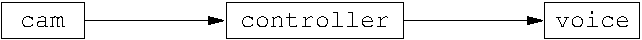
\includegraphics[scale=0.9]{figures/architecture}
\end{center}
\medskip

{\small
\begin{verbatim}
$ python cam/chesseye.py --src=1 \
    | controller/controller -kibbitz 1 \
    | python voice/speak.py
\end{verbatim}
}

\end{frame}


%%%%%%%%%%%%%%%%%%%%%%%%%%%%%%%%%%%%%%%%%%%%%%%%%%%%%%%%%%%%%%%%%%%%%%%%%%%
\section{Vision}
%%%%%%%%%%%%%%%%%%%%%%%%%%%%%%%%%%%%%%%%%%%%%%%%%%%%%%%%%%%%%%%%%%%%%%%%%%%

\begin{frame}[fragile]
\frametitle{Vision}

\vfill

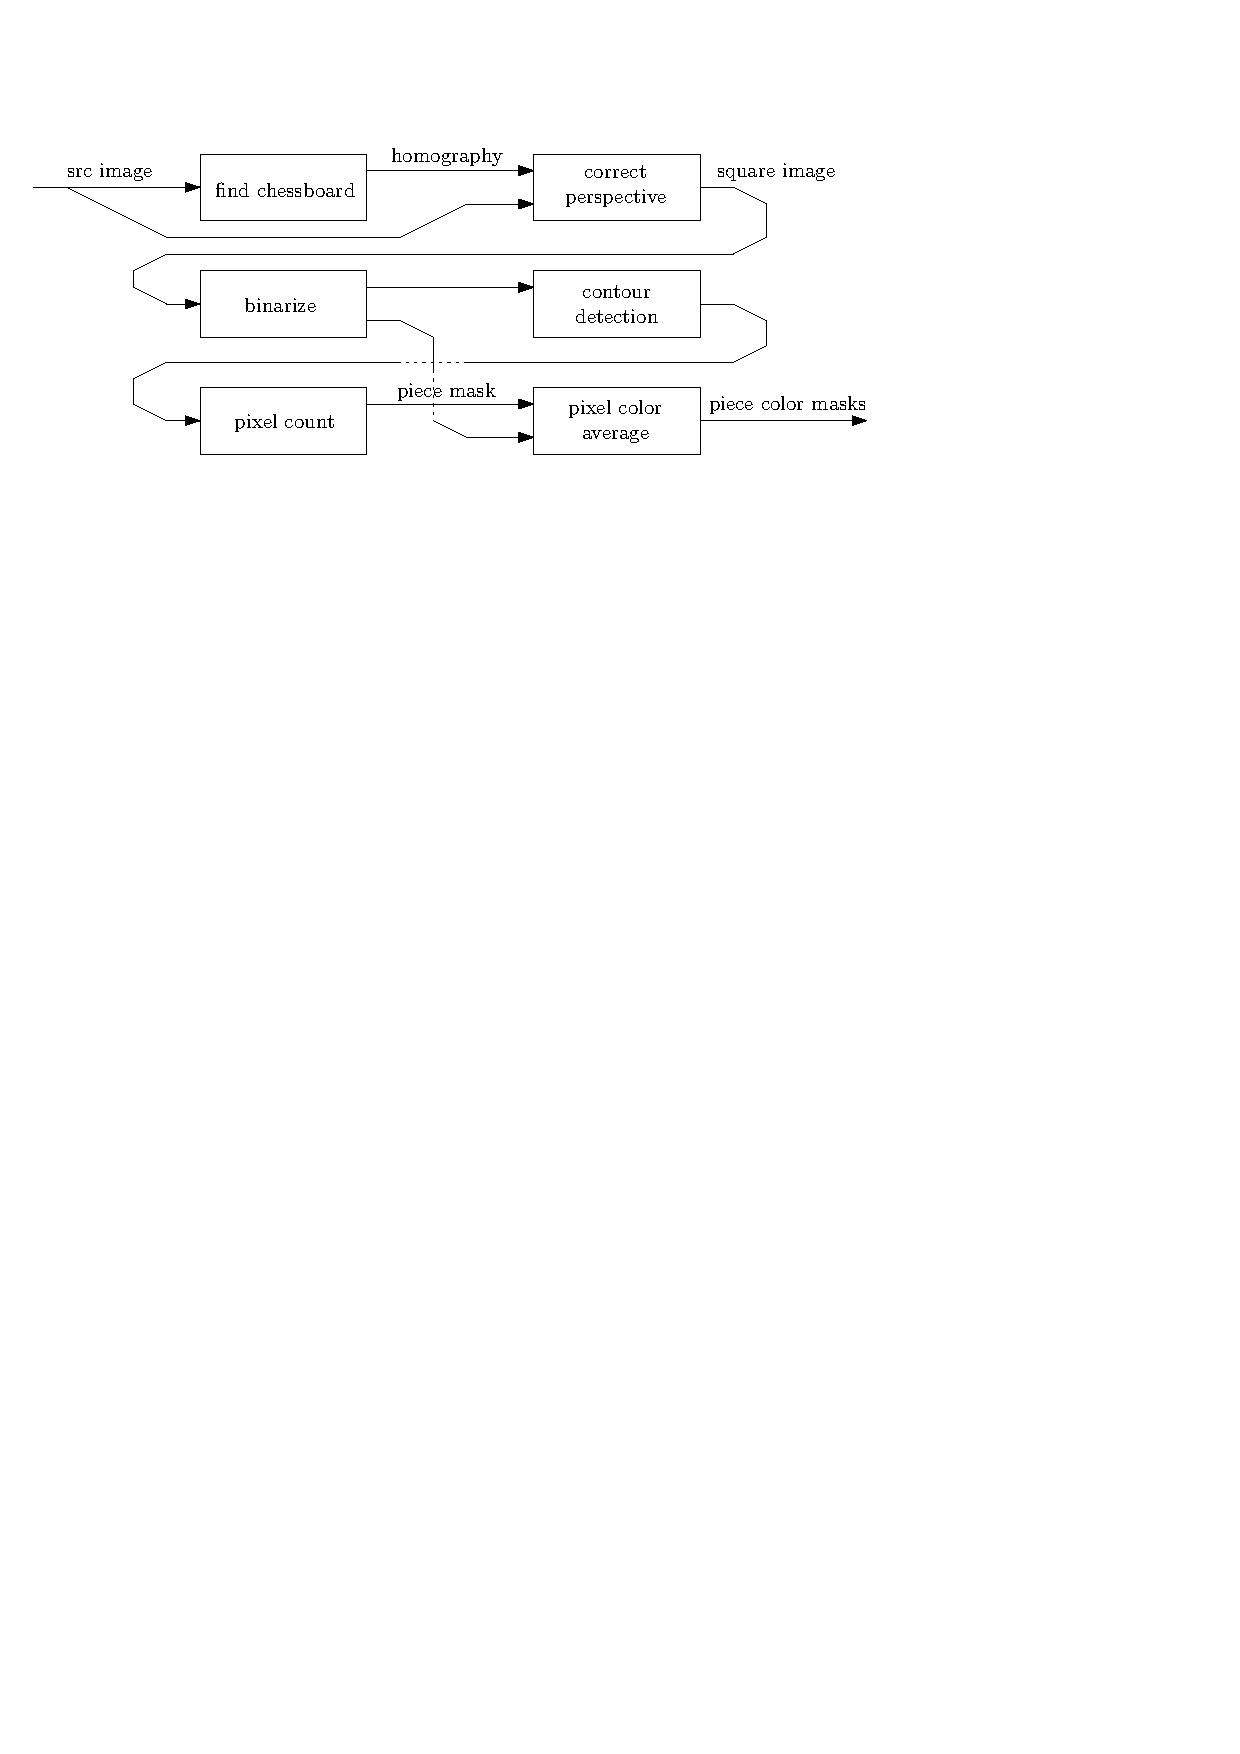
\includegraphics[scale=0.8]{figures/diagram}

\vfill

\end{frame}


%%%%%%%%%%%%%%%%%%%%%%%%%%%%%%%%%%%%%%%%%%%%%%%%%%%%%%%%%%%%%%%%%%%%%%%%%%%
\section{Controller}
%%%%%%%%%%%%%%%%%%%%%%%%%%%%%%%%%%%%%%%%%%%%%%%%%%%%%%%%%%%%%%%%%%%%%%%%%%%

\begin{frame}[fragile]
\frametitle{Controller}

XXX TODO Jerome XXX

\end{frame}

%%%%%%%%%%%%%%%%%%%%%%%%%%%%%%%%%%%%%%%%%%%%%%%%%%%%%%%%%%%%%%%%%%%%%%%%%%%

\begin{frame}[fragile]
\frametitle{Controller: architecture}

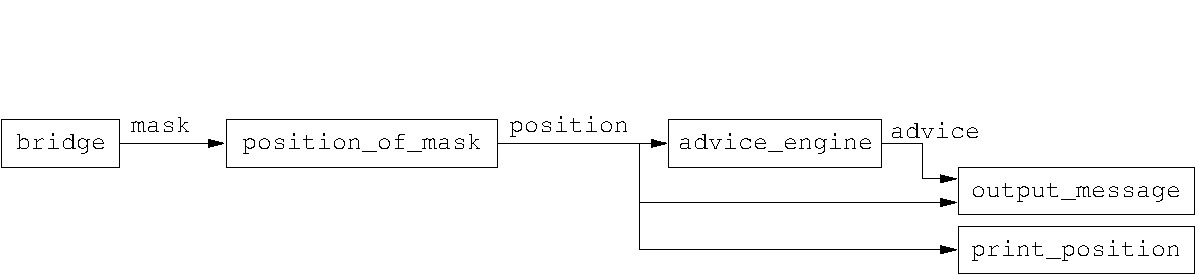
\includegraphics[scale=0.6]{figures/controller}

\pause

\begin{lstrml}
  signal mask default None gather keep_last in
  signal position default None gather keep_last in
  signal advice default None gather keep_last in
  begin
    run Bridge.bridge_async mask ||
    run position_of_mask mask position Ochess.init_position ||
    run advice_engine position advice ||
    run output_messages position advice ||
    run print_position position
  end
\end{lstrml}

\end{frame}

%%%%%%%%%%%%%%%%%%%%%%%%%%%%%%%%%%%%%%%%%%%%%%%%%%%%%%%%%%%%%%%%%%%%%%%%%%%

\begin{frame}[fragile]
\frametitle{Controller: example of process}

\begin{lstrml}
let process output_messages position advice =
  loop
    await position (Some (move, pos)) in
    print_endline ("MOVD "^(Ochess.long_string_of_move move pos));
    match Ochess.game_status pos with
    | Ochess.Win color -> print_endline "ENDG checkmate"
    | Ochess.Draw -> print_endline "ENDG stalemate"
    | Ochess.Play _ -> ()
  end
  ||
  loop
    await advice (Some (pos, smove)) in
    let msg = Ochess.long_string_of_smove pos smove in
    print_endline ("KIBB "^msg)
  end
\end{lstrml}

\end{frame}

%%%%%%%%%%%%%%%%%%%%%%%%%%%%%%%%%%%%%%%%%%%%%%%%%%%%%%%%%%%%%%%%%%%%%%%%%%%

\begin{frame}[fragile]
\frametitle{Controller}

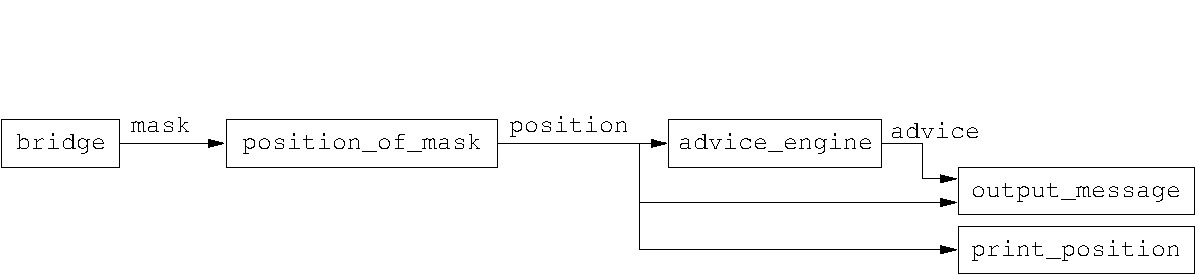
\includegraphics[scale=0.6]{figures/controller}

\begin{lstrml}
  signal mask default None gather keep_last in
  signal position default None gather keep_last in
  signal advice default None gather keep_last in
  begin
    run Bridge.bridge_async mask ||
    run position_of_mask mask position Ochess.init_position ||
    run advice_engine position advice ||
    run output_messages position advice ||
    run print_position position
  end
\end{lstrml}

\end{frame}

%%%%%%%%%%%%%%%%%%%%%%%%%%%%%%%%%%%%%%%%%%%%%%%%%%%%%%%%%%%%%%%%%%%%%%%%%%%

\begin{frame}[fragile]
\frametitle{Controller with reset}

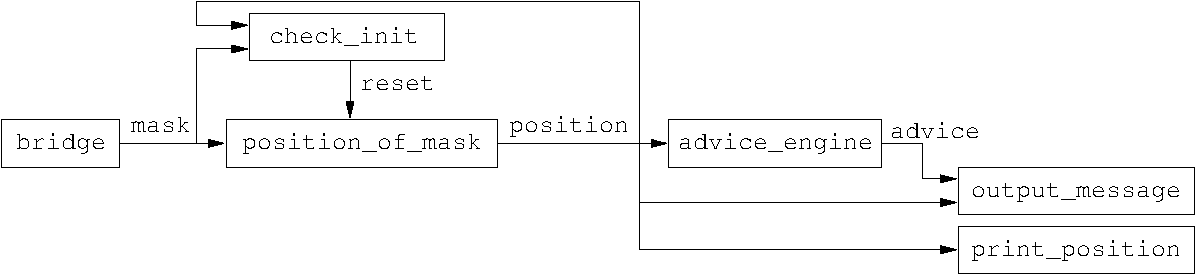
\includegraphics[scale=0.6]{figures/controller-with-reset}

\begin{lstrml}
  signal mask default None gather keep_last in
  signal position default None gather keep_last in
  signal advice default None gather keep_last in
  signal reset default () gather (fun () () -> ()) in
  begin
    run Bridge.bridge_async mask ||
    loop
      do
        run position_of_mask mask position Ochess.init_position
      until reset done
    end ||
    run check_init position mask reset ||
    ...
  end
\end{lstrml}

\end{frame}


%%%%%%%%%%%%%%%%%%%%%%%%%%%%%%%%%%%%%%%%%%%%%%%%%%%%%%%%%%%%%%%%%%%%%%%%%%%
\section{Voice}
%%%%%%%%%%%%%%%%%%%%%%%%%%%%%%%%%%%%%%%%%%%%%%%%%%%%%%%%%%%%%%%%%%%%%%%%%%%

\begin{frame}[fragile]
\frametitle{Voice}


\end{frame}

%%%%%%%%%%%%%%%%%%%%%%%%%%%%%%%%%%%%%%%%%%%%%%%%%%%%%%%%%%%%%%%%%%%%%%%%%%%
\section{Deliverable}
%%%%%%%%%%%%%%%%%%%%%%%%%%%%%%%%%%%%%%%%%%%%%%%%%%%%%%%%%%%%%%%%%%%%%%%%%%%

\begin{frame}[fragile]
\frametitle{Deliverable}

\begin{center}
  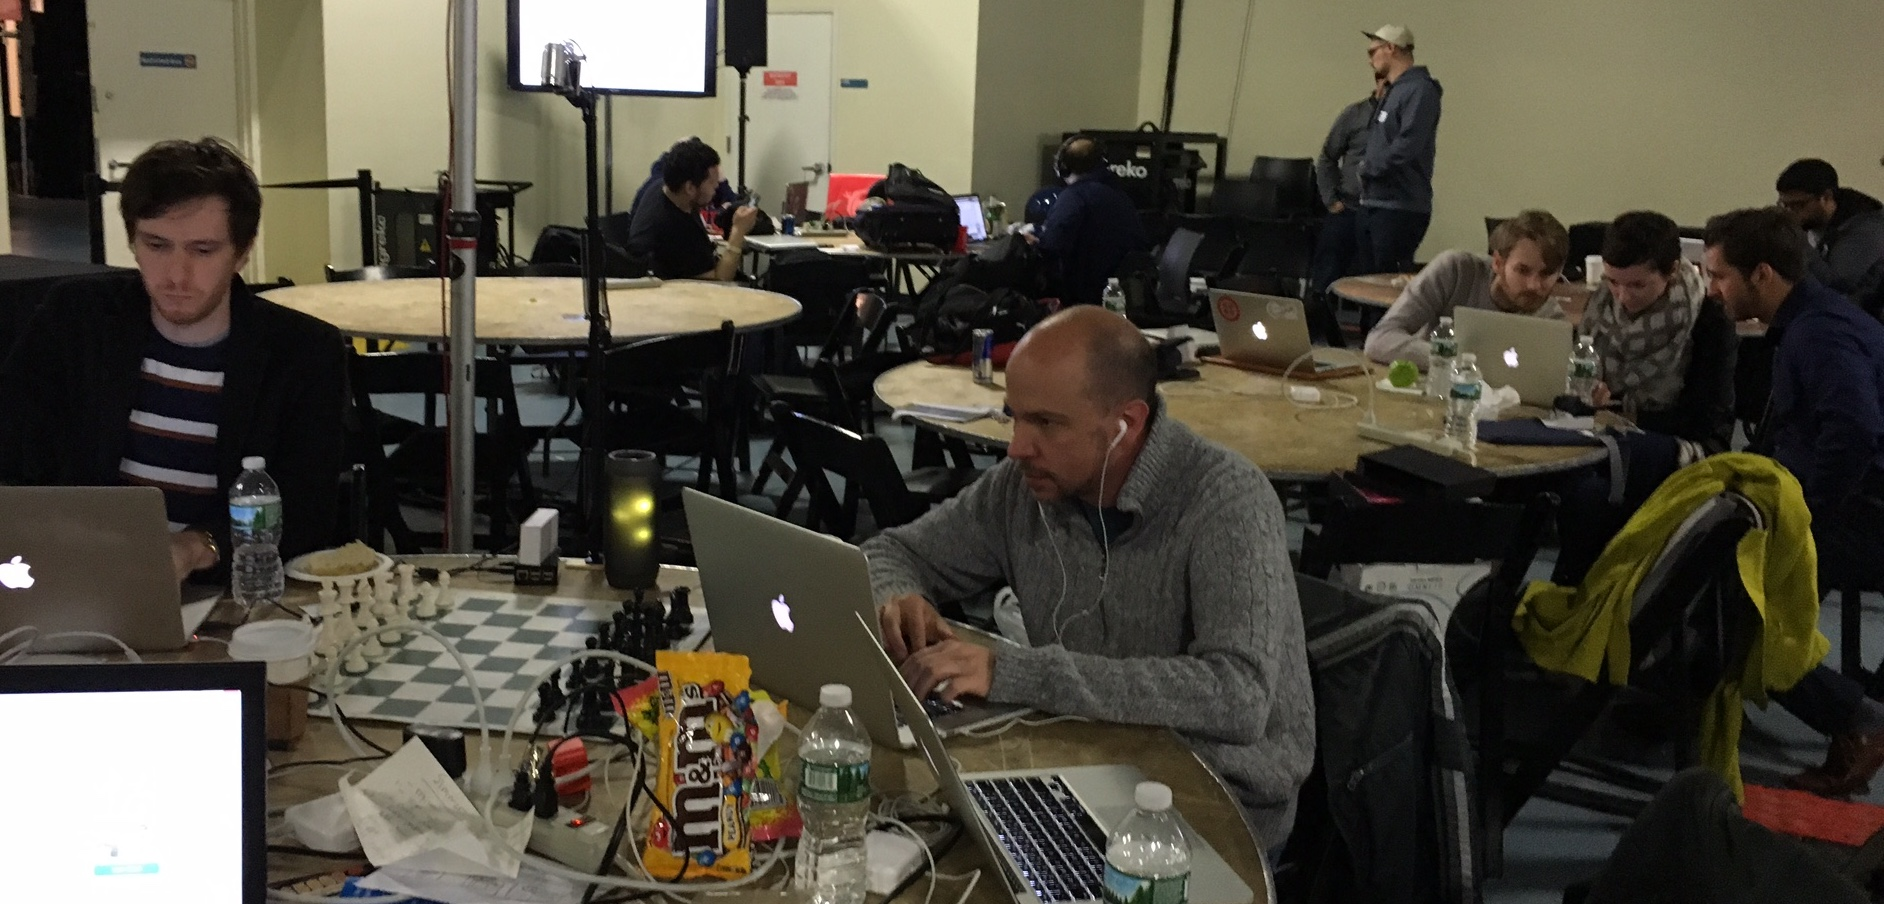
\includegraphics[scale=0.15]{figures/photo-deliverable}
\end{center}

\begin{itemize}
\item Source code: \url{https://github.com/chesseye/chesseye}
  \medskip
\item Web site: \url{http://devpost.com/software/chesseye}
  \medskip
\item Talk: \url{https://youtu.be/bYtGw61YLRk}
  \begin{itemize}
  \item background video: \url{https://vimeo.com/165765674}
  \end{itemize}
\end{itemize}


\end{frame}

% %%%%%%%%%%%%%%%%%%%%%%%%%%%%%%%%%%%%%%%%%%%%%%%%%%%%%%%%%%%%%%%%%%%%%%%%%%%

% \begin{frame}[fragile]
% \frametitle{}


% \end{frame}




\end{document}

%%% Local Variables:
%%% mode: pdflatex
%%% TeX-master: "cours"
%%% End:
